%-------------------------------------------------------------------------
% Design Project Input/Output Module Description
%-------------------------------------------------------------------------

\clearpage
\section{LED Matrix Output Module}
\label{sec-output-ledmatrix}

This output module enables your IoT device to control a 16x24 LED matrix
which can display useful messages and graphics on its large screen; for
example, the matrix can display digital clocks, thermometers, counters
and meters, instrumentation readouts, industrial control indicators,
etc. You can also chain multiples of these displays together! The panel
works using a special HT1632C chip on the back which does most of the
necessary work to display messages for you. Communication with the
matrix happens through a 3-pin serial interface which is easy to work
with.

A sample circuit and Arduino code is shown below to get you started.
The LED matrix has a gray ribbon connector that has a "red strip" on one
side of it. When connecting wires to the connector, the red wire for
power will be on the same side as the "red strip" on the ribbon
connector. The example code will draw pixels, rectangles, lines,
circles, and text messages on the screen. After setting up the circuit
and programming the Arduino, check that the shape/message appears on
screen correctly. You can now experiment with drawing moving shapes or
even scrolling text!

\vspace{0.1in}
\begin{minipage}[t]{0.49\tw}
  \vspace{0.0in}
  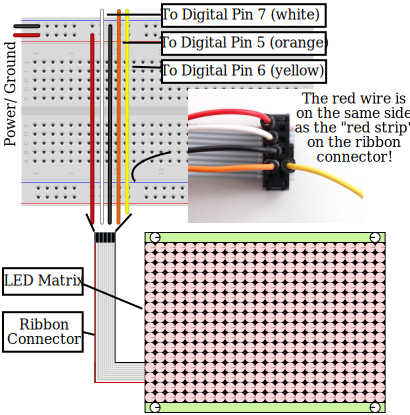
\includegraphics[width=\tw]{output-ledmatrix-annotated.svg.pdf}
\end{minipage}
\hspace{0.1in}
\begin{minipage}[t]{0.49\tw}
  \vspace{0.1in}
  \begin{Verbatim}[gobble=3,fontsize=\small]
    #include "HT1632.h"

    int pin_data = 5; // orange wire
    int pin_wr   = 6; // yellow wire
    int pin_cs   = 7; // white wire

    HT1632LEDMatrix matrix =
      HT1632LEDMatrix(pin_data, pin_wr, pin_cs);

    void setup() {
      Serial.begin(9600);
      matrix.begin(HT1632_COMMON_16NMOS);
      matrix.fillScreen();
      delay(500);
    }

    void loop() {
      matrix.clearScreen();

      // Draw pixels with:
      // - drawPixel( x_coordinate, y_coordinate, value )
      // In this example, we draw a pixel at point (0, 0),
      // delay 500 ms, clear the pixel, and wait another
      // 500 ms.

      matrix.drawPixel(0, 0, 1); // value 1 lights LED
      matrix.writeScreen();
      delay(500);
      matrix.drawPixel(0, 0, 0); // value 0 turns off LED
      delay(500);

      //// Draw rectangle outlines with:
      // - drawRect( x_coordinate, y_coordinate,
      //             rectangle_width, rectangle_height,
      //             value )
      // In this example, we draw a rectangle at point
      // (6, 4), that is half the width and half the
      // height of the entire matrix. Then we clear it.
      // Use "fillRect" to draw a filled rectangle.

      matrix.drawRect(6, 4,
                matrix.width()/2, matrix.height()/2, 1);
      matrix.writeScreen();
      delay(500);
      matrix.clearScreen();
      delay(500);

      // Draw lines with:
      // - drawLine( x1_coordinate, y1_coordinate,
      //             x2_coordinate, y2_coordinate,
      //             value )
      // In this example, we draw an X and then clear it.

      matrix.drawLine(0, 0,
                matrix.width()-1, matrix.height()-1, 1);
      matrix.drawLine(matrix.width()-1, 0,
                0, matrix.height()-1, 1);
      matrix.writeScreen();
      delay(500);
      matrix.clearScreen();
      delay(500);

      // Draw circles with:
      // - drawCircle( x_coordinate, y_coordinate,
      //               radius, value )
      // The coordinates are for the center of the
      // circle. In this example we draw a circle and
      // clear it. Use "fillCircle" to draw a filled
      // circle instead.

      matrix.drawCircle(
                matrix.width()/2-1, matrix.height()/2-1,
                8, 1);
      matrix.writeScreen();
      delay(500);
      matrix.clearScreen();
      delay(500);

      // Draw text with:
      // - matrix.setCursor(x_coordinate, y_coordinate)
      // - matrix.print( text_to_print )
      // In this example, we draw two lines of text!

      matrix.setTextSize(1);  // size 1 == 8 pixels high
      matrix.setTextColor(1); // 'lit' LEDs

      matrix.setCursor(0, 0); // start at top left
      matrix.print("Curi");
      matrix.setCursor(0, 8); // next line, 8 pixels down
      matrix.print("e'14");
      matrix.writeScreen();
      delay(500);
      matrix.clearScreen();
      delay(500);

    }
  \end{Verbatim}
\end{minipage}
\vspace{0.1in}

%Questions:
